\documentclass[10pt,aspectratio=169]{beamer}

%% Fonts
\usepackage{multicol}
\usepackage{mathabx}
\usepackage[scaled]{helvet}
\usepackage{lmodern}
\usepackage{eulervm}
\usepackage{natbib}
\usepackage{booktabs}
\usepackage{amsfonts}
%\usepackage{multicol}
%\usefonttheme[onlymath]{serif}
%\usefonttheme{professionalfonts}
\usefonttheme{structurebold}
\usepackage{bm}


%% Color & Theme
\definecolor{SUblue}{RGB}{0,0,180}
\usecolortheme[RGB={0,0,180}]{structure}
\usetheme{Boadilla}
\setbeamertemplate{navigation symbols}{}
\setbeamertemplate{itemize items}[circle]
\setbeamertemplate{enumerate items}[circle]
\setbeamerfont{title}{size=\large}
\setbeamerfont{frametitle}{size=\large}
\setbeamerfont{framesubtitle}{size=\large,shape =$\color{violet}{\looparrowdownright}~$}
\setbeamercolor{title}{fg=white, bg= SUblue!75!green}
\setbeamercolor{framesubtitle}{fg=violet}
%% \setlength{\leftmargini}{5pt}

\hypersetup{
  colorlinks=true,
  linkcolor=SUblue,
  citecolor=SUblue,
  urlcolor=SUblue}


\title[Covariate-Dependent Copula Modeling]{\textbf{Bayesian covariate-dependent copula
    modeling\\ --- with applications in stocks, text sentiments and firm credit risks}}



\author[Feng Li]{%\includegraphics[height=2cm]{cufelogo}\\
  \vspace{0.5cm}\textbf{Feng Li}
  \\\vspace{0.3cm}\url{feng.li@cufe.edu.cn}\\\url{http://feng.li/}}

\institute[SAM.CUFE.EDU.CN]{\footnotesize{\textbf{School of Statistics and
      Mathematics\\ Central University of Finance and Economics}}}
\date{}

\begin{document}
%% Title page
\begin{frame}[plain]
  \addtocounter{framenumber}{-1}
  \titlepage
\end{frame}

\section*{Outline}
\begin{frame}
  \frametitle{Outline}
  \addtocounter{framenumber}{-1}
  \tableofcontents
\end{frame}


\begin{frame}
  \frametitle{Collaborators on the series of papers}
  \begin{itemize}
  \item Yanfei Kang, Associate Professor, Beihang University, Beijing China.
  \item Zhuojing He, PhD student, Central University of Finance and Economics, Beijing
    China.
  \item Anastasios Panagiotelis, Associate Professor, Monash University, Australia.

    \vspace{2cm} \color{blue} \item [*] Feng Li's research is supported by National
    Natural Science Foundation of China.

  \end{itemize}


\end{frame}


\section{Covariate-dependent copula models}


% \begin{frame}
%   \frametitle{What is a copula?}
%   \begin{itemize}
%   \item The word ``copula'' means \textbf{linking}.
%   \item \textbf{Sklar's theorem}

%     Let $H$ be a multi-dimensional distribution function with marginal
%     distribution functions $F_1(x_1),...,F_m(x_m)$. Then there exists a
%     function $C$ (\textbf{copula function}) such that
%     \begin{equation*}
%       \begin{split}
%         H(x_1,...,x_m)= & C(F_1(x_1),...,F_m(x_m))\\
%         =&C\left(\int_{-\infty}^{x_1}f(z_1)dz_1,...,\int_{-\infty}^{x_m}f(z_m)dz_m\right)=C(u_1,...,u_m).
%       \end{split}
%     \end{equation*}
%     Furthermore, if $F_i(x_i)$ are continuous, then $C$ is unique, and the derivative $c(u_1,...,u_m)= \partial^m C(u_1,...,u_m)/(\partial u_1...
%     \partial u_m)$ is the \textbf{copula density}.

%   \end{itemize}
% \end{frame}



\begin{frame}
  \frametitle{Covariate-dependent copula models}
  \framesubtitle{The Joe-Clayton copula example}
  \begin{itemize}
  \item The Joe-Clayton copula function
    \[
    \begin{split}
      C(u,v,\theta,\delta)=&1-\left[1-\left\{\left(1-\bar u ^{\theta }\right)^{-\delta
          }+\left(1-\bar v ^{\theta }\right)^{-\delta }-1\right\}^{-1/\delta
        }\right]^{1/\theta }
    \end{split}
    \]
    where $\theta \geq 1$, $\delta > 0$, $\bar u = 1-u$, $\bar v = 1-v$ .

  \item Some properties:
    \begin{itemize}

    \item $\lambda_L=2^{-1/\delta}$ does not depend on $\lambda_U=2-2^{-1/\theta}$.
    \item  $\tau=1- 4\int _0^{\infty} s\times(\varphi'(s))^2ds$ is calculated via Laplace transform.
    \end{itemize}
  \end{itemize}

\end{frame}


\begin{frame}
  \frametitle{Covariate-dependent copula models}
  \framesubtitle{The reparameterized copula model}
  \begin{itemize}

  % \item \textbf{The motivation} i) The interpretation of correlation and tail-dependence.
  %   ii) Dynamical modeling tail-dependence and correlation.

  \item \textbf{Reparametrization}: We reparameterize the copula as a function of
    tail-dependence and/or Kendall's tau $C(\bm{u},\lambda_L,\tau)$.

  \item \textbf{Link with covariates}: All copula features in the $k$:th and $l$:th margins can be connected with
    covariates
      \begin{align*}
        \tau_{kl}&=l_{\tau}^{-1}(\bm{X}_{kl}\bm{\beta}_{\tau}),\\
        \lambda_{kl}&=l_{\lambda}^{-1}(\bm{X}_{kl}\bm{\beta}_{\lambda})
      \end{align*}

    \item \textbf{Applicable Copulas}: Any copula can be equally well used with such
      reparameterization when there is closed form of tail-dependence and Kendall's
      $\tau$.

    \begin{itemize}
    \item \textbf{Archimedean copulas}: Joe-Clayton, Clayton, Gumbel,...
    \item \textbf{Elliptical copulas}: Gaussian and \emph{t} copulas
    \end{itemize}

  \item Marginal models we have used

    \begin{itemize}
    \item Mixture of asymmetric student's-\emph{t} distributions.
    \item GARCH models
    \item stochastic volatility (SV) models.
    \item Poisson regression models.
    \end{itemize}

  \end{itemize}
\end{frame}

\section{The Bayesian scheme}


\begin{frame}%[allowframebreaks]
  \frametitle{The Bayesian approach}
  \begin{itemize}

  \item \textbf{The log Posterior}
    \[
    \begin{split}\log p(\{\bm{\beta},\bm{\mathcal{I}}\}|\bm{y},\bm{x})=
      \mathrm{c}&+\sum\nolimits _{j=1}^{M}\left\{\log
        p(\bm{y}_{.j}|\{\bm{\beta},\bm{\mathcal{I}}\}_{j},\bm{x}_{j}) + \log p(\{\bm{\beta},\bm{\mathcal{I}}_j\}) \right\}\\
      & +\log\mathcal{L}_{C}(\bm{u}_{1:M}|\{\bm{\beta},\bm{\mathcal{I}}\}_{C},\bm{y},\bm{x})+
      \log p_C(\{\bm{\beta},\bm{\mathcal{I}}\})
    \end{split}
    \]

    where
    \begin{itemize}
    \item $\{\bm{\beta}\}$ are the coefficient in the linking function,
    \item $\{\bm{\mathcal{I}}\}$ are the corresponding variable selection indicators.
    \item $\{\bm{\beta},\bm{\mathcal{I}}\}$ can be estimated jointly via Bayesian approach.
    \item $\bm{u}_{j}=F_{j}(y_{j})$ is the CDF of the $j$:th marginal model.
    \end{itemize}

    % \begin{equation*}
    %   \begin{split}
    %     & \log \mathcal{L} (Y_u,Y_v| X_u, X_v,\lambda_L, \tau,\beta_u,\beta_v) =  \sum_{i=1}^{n}
    %     \log c(u_i,v_i, \lambda_L, \tau) \\
    %     & \hspace{2.8cm}  + \log \mathcal{L}_u(Y_u|X_u,\beta_u) + \log \mathcal{L}_v(Y_v|X_v,\beta_v)\\
    %   \end{split}
    % \end{equation*}

  \end{itemize}
\end{frame}


\begin{frame}
  \frametitle{The Bayesian approach}
  \begin{itemize}

  \item \textbf{The priors} for the copula model are easy to specify due to our
    reparameterization.

    \begin{itemize}

    \item It it \textbf{not easy} to specify priors directly on
      $\{\bm{\beta},\bm{\mathcal{I}}\}$

    \item But it is \textbf{easy} to puts prior information on the model parameters
      features ($\tau$, $\mu$, $\sigma^2$) and then derive the implied prior on the
      intercepts and variable selection indicators.

    \item When variable selection is used, we assume there are no covariates in
      the link functions \emph{a priori}.

    \end{itemize}

  \item \textbf{The posterior} inference is straightforward although the model is very
    complicated.
  \end{itemize}
\end{frame}

\begin{frame}%[allowframebreaks]
  \frametitle{The Bayesian approach}
  \framesubtitle{Sampling the posterior with an efficient MCMC scheme}
  \begin{itemize}
  \item We update all the parameters \textbf{jointly} by using tailored
    Metropolis-Hastings within Gibbs. This is more efficient compared to the two-stage
    inference according to our study.

  \item \textbf{Taming the Beast:} the analytical gradients require the derivative for the
    copula density and marginal densities which can be conveniently decomposed via the
    chain rule that greatly reduces the complexity of the the gradient calculation.


  \item \textbf{Bayesian variable selection} is carried out simultaneously.

    % \item It is eventually straightforward. Thanks to the chain rule!

  % \end{itemize}


  % \begin{itemize}
  \item The Gibbs sampler for covariate-dependent copula.
  % \item The notation $\{\beta_{\mu},\mathcal{I}_{\mu}\}_{-m}$ indicates all other
  %   parameters in the model except $\{\beta_{\mu},\mathcal{I}_{\mu}\}_{m}$. The updating
  %   order is column-wise from left to right. If dependent link functions are used, the
  %   updating should be ordered accordingly.
  \begin{table}
    \label{tab:gibbs}
    \centering
    \resizebox{0.9 \textwidth}{!}{
      \begin{tabular}{llll}
        \toprule
        Margin component $(1)$ & ...  & Margin component ($M$) & Copula component ($C$)\tabularnewline
                                                                 \midrule
                                                                 $(1.1)$ $\{\beta_{\mu},\mathcal{I}_{\mu}\}_{1}|\{\beta_{\mu},\mathcal{I}_{\mu}\}_{-1}$  & ...  & $(M.1)$ $\{\beta_{\mu},\mathcal{I}_{\mu}\}_{M}|\{\beta_{\mu},\mathcal{I}_{\mu}\}_{-M}$  & $(C.1)$ $\{\beta_{\lambda},\mathcal{I}_{\lambda}\}_{C}|\{\beta_{\lambda},\mathcal{I}_{\lambda}\}_{-C}$\tabularnewline
                                                                                                                                                                                                                                                            $(1.2)$ $\{\beta_{\phi},\mathcal{I}_{\phi}\}_{1}|\{\beta_{\phi},\mathcal{I}_{\phi}\}_{-1}$  & ...  & $(M.2)$ $\{\beta_{\phi},\mathcal{I}_{\phi}\}_{M}|\{\beta_{\phi},\mathcal{I}_{\phi}\}_{-M}$  & $(C.2)$ $\{\beta_{\tau},\mathcal{I}_{\tau}\}_{C}|\{\beta_{\tau},\mathcal{I}_{\tau}\}_{-C}$\tabularnewline
                                                                                                                                                                                                                                                                                                                                                                                                                                                               $(1.3)$ $\{\beta_{\nu},\mathcal{I}_{\nu}\}_{1}|\{\beta_{\nu},\mathcal{I}_{\nu}\}_{-1}$  & ...  & $(M.3)$ $\{\beta_{\nu},\mathcal{I}_{\nu}\}_{M}|\{\beta_{\nu},\mathcal{I}_{\nu}\}_{-M}$  & \tabularnewline
                                                                                                                                                                                                                                                                                                                                                                                                                                                                                                                                                                                                                                                          $(1.4)$ $\{\beta_{\kappa},\mathcal{I}_{\kappa}\}_{1}|\{\beta_{\kappa},\mathcal{I}_{\kappa}\}_{-1}$  & ...  & $(M.4)$ $\{\beta_{\kappa},\mathcal{I}_{\kappa}\}_{M}|\{\beta_{\kappa},\mathcal{I}_{\kappa}\}_{-M}$  & \tabularnewline
                                                                                                                                                                                                                                                                                                                                                                                                                                                                                                                                                                                                                                                                                                                                                                                                                                                                             \bottomrule
      \end{tabular}
    }
  \end{table}
\end{itemize}

\end{frame}


% \begin{frame}
%   \frametitle{The Bayesian approach}
%   \framesubtitle{Why not two-stage approach?}
%   \begin{itemize}
%   \item The asymptotic relative efficiency of the two-stage estimation procedure depends
%     on how close the copula is to the Fr\'echet bounds
%     {\citep{joe2005asymptotic}}.
%   \item The two-stage approach in estimating the multivariate DCC GARCH model is
%     consistent but not fully efficient due to the limited information provided by the
%     estimators {\citep{engle2001theoretical}}.
%   \end{itemize}
% \end{frame}

\begin{frame}
  \frametitle{Model Comparison}
  \begin{itemize}
  \item We evaluating the model performance based on \textbf{out-of-sample prediction}.
  \item In our time series application, we estimate the model based on the 80\% of
    historical data and then predict the last 20\% data.

  \item We evaluate the quality of the one-step-ahead predictions using the \textbf{log
      predictive score} (LPS)
    \begin{align*}
      \mathrm{LPS}=&\log p(D_{(T+1):(T+p)}|D_{1:T})\\
      =&\sum\nolimits _{i=1}^{p}\log\int p(D_{T+i}|\theta,D_{1:(T+i-1)})p(\theta|D_{1:(T+i-1)})\mathrm{d}\theta
    \end{align*}
    where $D_{a:b}$ is the dataset from time $a$ to $b$ and $\theta$ are the model
    parameters.
  \end{itemize}
\end{frame}


\begin{frame}
  \frametitle{Simulation}

  \begin{figure}[!h]
    \centering
    \includegraphics[width=0.8\textwidth]{LPDSComp}
  \end{figure}
\end{frame}

\begin{frame}
  \frametitle{Simulation}

  \begin{figure}[!h]
    \centering
    \includegraphics[width=0.48\textwidth]{DGP}
  \end{figure}
\end{frame}


\begin{frame}
  \frametitle{Improving forecasting performance with covariate-dependent tail-dependence
    (Li \& Kang, 2016)}

  \framesubtitle{Log predictive density score comparison}
  \begin{table}
  % \caption{A model comparison with the LPS. Note that variable selection is used in all
  %   situations in the margins. $C(CD.)$ indicates the covariate-contingent structure used
  %   in the reparameterized copula component, and $C(Const.)$ means only constant
  %   tail-dependence and correlation are estimated in the copula component. Note that in
  %   principle, the global LPS should be equal to the summation of LPSs in the marginal and
  %   copula components. Due to MCMC numerical errors, the results are not exactly the
  %   same. The numerical standard errors are all below one in all LPSs. The LPS for the
  %   Joe-Clayton copula $C(\lambda_L,\tau)$ is the same as $C(\lambda_L,\lambda_U)$.}
  \label{tab:lpds}
  \begin{center}
     \resizebox{0.4\columnwidth}{!}{%
    \begin{tabular}{llrrrr}
      \toprule

      &&\multicolumn{4}{c}{Reparameterized Copulas}\\
      \cline{3-6}
      &&Joe-Clayton&Clayton&Gumbel&\emph{t}-Copula\\

      Margins&\multicolumn{1}{c}{LPS decomposition}&&&&\\
      % \multicolumn{2}{c}{ComponentsCombination}
      % \multicolumn{2}{c}{}&$(\lambda_L,~\lambda_U)$&$(\tau)$&$(\tau)$&$(\tau,~\nu)$\\

      \midrule

      \multicolumn{6}{c}{(\emph{Joint modeling approach})}\\

      SPLIT-\emph{t}&$M_1$&$-1743.12$&$-1741.04$&$-1754.36$&$-1741.47$\\
      &$M_2$&$-1435.98$&$-1468.25$&$-1485.68$&$-1430.07$\\
      &$C(CD.)$&$837.50$&$690.22$&$797.78$&${792.14}$\\
      % \cline{1-2}
      &$Global$&${-2344.12}$&$-2523.75$&$-2448.14$&$-2380.12$\\
      \\

      SPLIT-\emph{t}&$M_1$&$-1747.99$&$-1747.15$&$-1754.61$&$-1782.37$\\
      &$M_2$&$-1434.22$&$-1449.95$&$-1446.84$&$-1658.09$\\
      &$C(Const.)$&$779.14$&$654.46$&$780.33$&${703.96}$\\
      % \cline{1-2}
      &$Global$&${-2411.06}$&$-2547.14$&$-2421.15$&$-2736.49$\\
      \midrule

      \multicolumn{6}{c}{(\emph{Two-stage modeling approach})}\\

      SPLIT-\emph{t}&$M_1$&$-1740.10$&$-1741.05$&$-1737.73$&$-1741.47$\\
      &$M_2$&$-1428.39$&$-1436.63$&$-1427.83$&$-1433.41$\\
      &$C(CD.)$&$819.63$&$694.84$&$781.39$&$788.22$\\
      % \cline{1-2}
      &$Global$&${-2346.61}$&$-2483.93$&$-2392.13$&$-2389.41$\\

      \\
      GARCH(1,1)&$M_1$&$-1948.07$&$-1948.07$&$-1948.07$&$-1948.07$\\
      &$M_2$&$-1673.85$&$-1673.85$&$-1673.85$&$-1673.85$\\
      &$C(CD.)$&$702.35$&$530.48$&$810.39$&$791.55$\\
      % \cline{1-2}
      &$global$&$-2919.57$&$$-3091.44$$&$-2811.53$&$-2830.37$\\
      \\
      SV&$M_1$&$-2166.90$&$-2154.18$&$-2168.17$&$-2179.36$\\
      &$M_2$&$-1811.36$&$-1844.57$&$-1808.61$&$-1808.24$\\
      &$C(CD.)$&$964.37$&$698.30$&$1012.10$&$1053.19$\\
      % \cline{1-2}
      &$Global$&$-3013.90$&$-3300.46$&$-2964.68$&$-2934.40$\\

      \midrule
      \multicolumn{6}{c}{(\emph{Bivariate volatility models})}\\

      \multicolumn{2}{l}{Bivariate DCC-GARCH}&$-2730.78$&\\
      \multicolumn{2}{l}{Bivariate SV}&$-2999.63$&\\
      \bottomrule
    \end{tabular}
     }
  \end{center}

\end{table}

\end{frame}

\section{Improving forecasting performance with covariate-dependent tail-dependence (Li \&
  Kang, 2016)}



\begin{frame}
  \frametitle{Improving forecasting performance with covariate-dependent tail-dependence (Li \&
  Kang, 2016)}
  \framesubtitle{The S\&P 100 and S\&P 600 and their empirical copulas}
 \begin{figure}[!h]
    \centering
    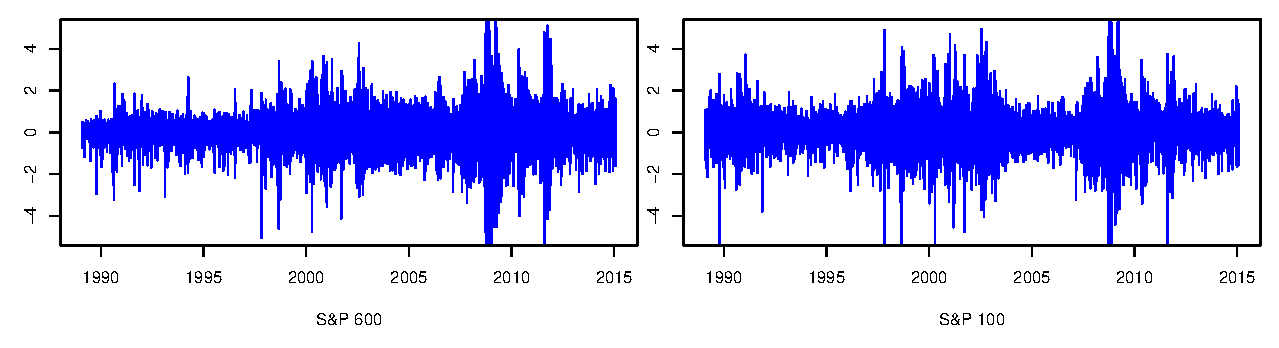
\includegraphics[width=0.5\textwidth]{SP100-SP600}\\
    \includegraphics[width=0.5\textwidth]{SP100-SP600-empCopula}
  \end{figure}
\end{frame}

\begin{frame}
  \frametitle{}

  \begin{figure}[!h]
    \frametitle{Contour plots of the posterior densities}
    \centering
    \includegraphics[width=0.45\textwidth]{Contour-Post}
  \end{figure}

\end{frame}

\section{Detecting credit risk clustering (Li \& He, 2017)}
\begin{frame}
  \frametitle{Detecting credit risk clustering with distance-to-default index \\(Li \& He,
    2017)}
  \begin{figure}[!h]
    \centering
    \includegraphics[width=0.6\textwidth]{DTD10ts}
    \caption{Distance-to-default (DTD) for 10 firms. In risk management, the probability of
      default is high if the value of DTD is small.}
    \label{fig:DTD-for-ten-firms}
  \end{figure}

\end{frame}

\newcommand{\tabincell}[2]{\begin{tabular}{@{}#1@{}}#2\end{tabular}}
\begin{frame}
  \frametitle{Covariates effects on the tail-dependency}
  \begin{table}
    % \caption{Covariates effects on the tail-dependency between \textsf{SZKFT} and
    %   \textsf{CGWC}.}
  \label{tab:driving-covariates-tail-dependence-coefficients-between-SZKFT-CGWC}
  \begin{center}
    \resizebox{0.6\textwidth}{!}{
    \begin{tabular}{lrrrrrrr}
      \toprule
      & \tabincell{l}{No \\ covariates} & & \tabincell{l}{Macroeconomic \\ covariates} & & \tabincell{l}{Specific \\ covariates} & & \tabincell{l}{Macroeconomic and \\ specific covariates} \\
      \midrule
      Constant  & $-4.931$  &  & $2.014$ &  & $-2.174$ &  & $10.515$  \\
      & $(1.000)$ &  & $(1.000)$  &  & $(1.000)$ &  & $(1.000)$  \\
      CPI       &  &  & $-0.431$  &   &  &  & $-71.814$  \\
      &  &  & $(0.593)$ &   &  &  &  $(0.507)$  \\
      M2 growth rate &  &  & $-0.122$  &  &  &  & $2.169$  \\
      &  &  & $(0.586)$ &  &  &  & $(0.636)$  \\
      Short-term interest rate &  &  & $-0.012$  &  &  &  & $11.998$  \\
      &  &  & $(0.988)$ &  &  &  & $(0.254)$  \\
      RMB/USD spot rate  &  &  & $-0.526$ &  &  &  & $-0.650$  \\
      &  &  & $(0.605)$  &  &  &  & $(0.309)$  \\
      \textsf{CGWC}'s solvency capacity  &  &  &  &  & $-0.017$  &  & $4.498$  \\
      &  &  &  &  & $(0.866)$ &  & $(0.590)$  \\
      \textsf{CGWC}'s developing capacity   &  &  &  &  & $0.012$   &  & $-1.680$  \\
      &  &  &  &  & $(0.637)$ &  & $(0.624)$  \\
      \textsf{CGWC}'s profitability  &  &  &  &  & $0.004$ &  & $-12.948$ \\
      &  &  &  &  & $(0.751)$  &  & $(0.597)$  \\
      \textsf{CGWC}'s operating capacity   &  &  &  &  & $-0.039$  &  & $4.819$ \\
      &  &  &  &  & $(0.716)$ &  & $(0.615)$ \\
      \textsf{XITG}'s solvency capacity  &  &  &  &  & $0.089$ &  & $58.419$ \\
      &  &  &  &  & $(0.813)$  &  & $(0.537)$  \\
      \textsf{XITG}'s developing capacity   &  &  &  &  & $0.030$ &  & $104.257$  \\
      &  &  &  &  & $(0.652)$ &  & $(0.578)$  \\
      \textsf{XITG}'s profitability  &  &  &  &  & $-0.409$  &  & $294.978$ \\
      &  &  &  &  & $(0.531)$ &  & $(0.389)$  \\
      \textsf{XITG}'s operating capacity   &  &  &  &  & $-0.057$  &  & $-0.305$ \\
      &  &  &  &  & $(0.857)$ &  & $(0.463)$  \\
      \midrule
      LPS  & $-308.732$ &  & $-200.606$ &  & $-106.542$ &  & $-52.831$   \\
      \bottomrule
    \end{tabular}
    }
  \end{center}
\end{table}

\end{frame}

\section{Multivariate covariate-dependence with mixed margins (Li, Panagiotelis \& Kang, ongoing
  research)}

\begin{frame}
  \frametitle{Multivariate covariate-dependence with mixed margins (Li, Panagiotelis \&
    Kang, ongoing research)}
  \framesubtitle{Modeling stock returns and text sentiments}
  \begin{figure}[!h]
    \centering
    % 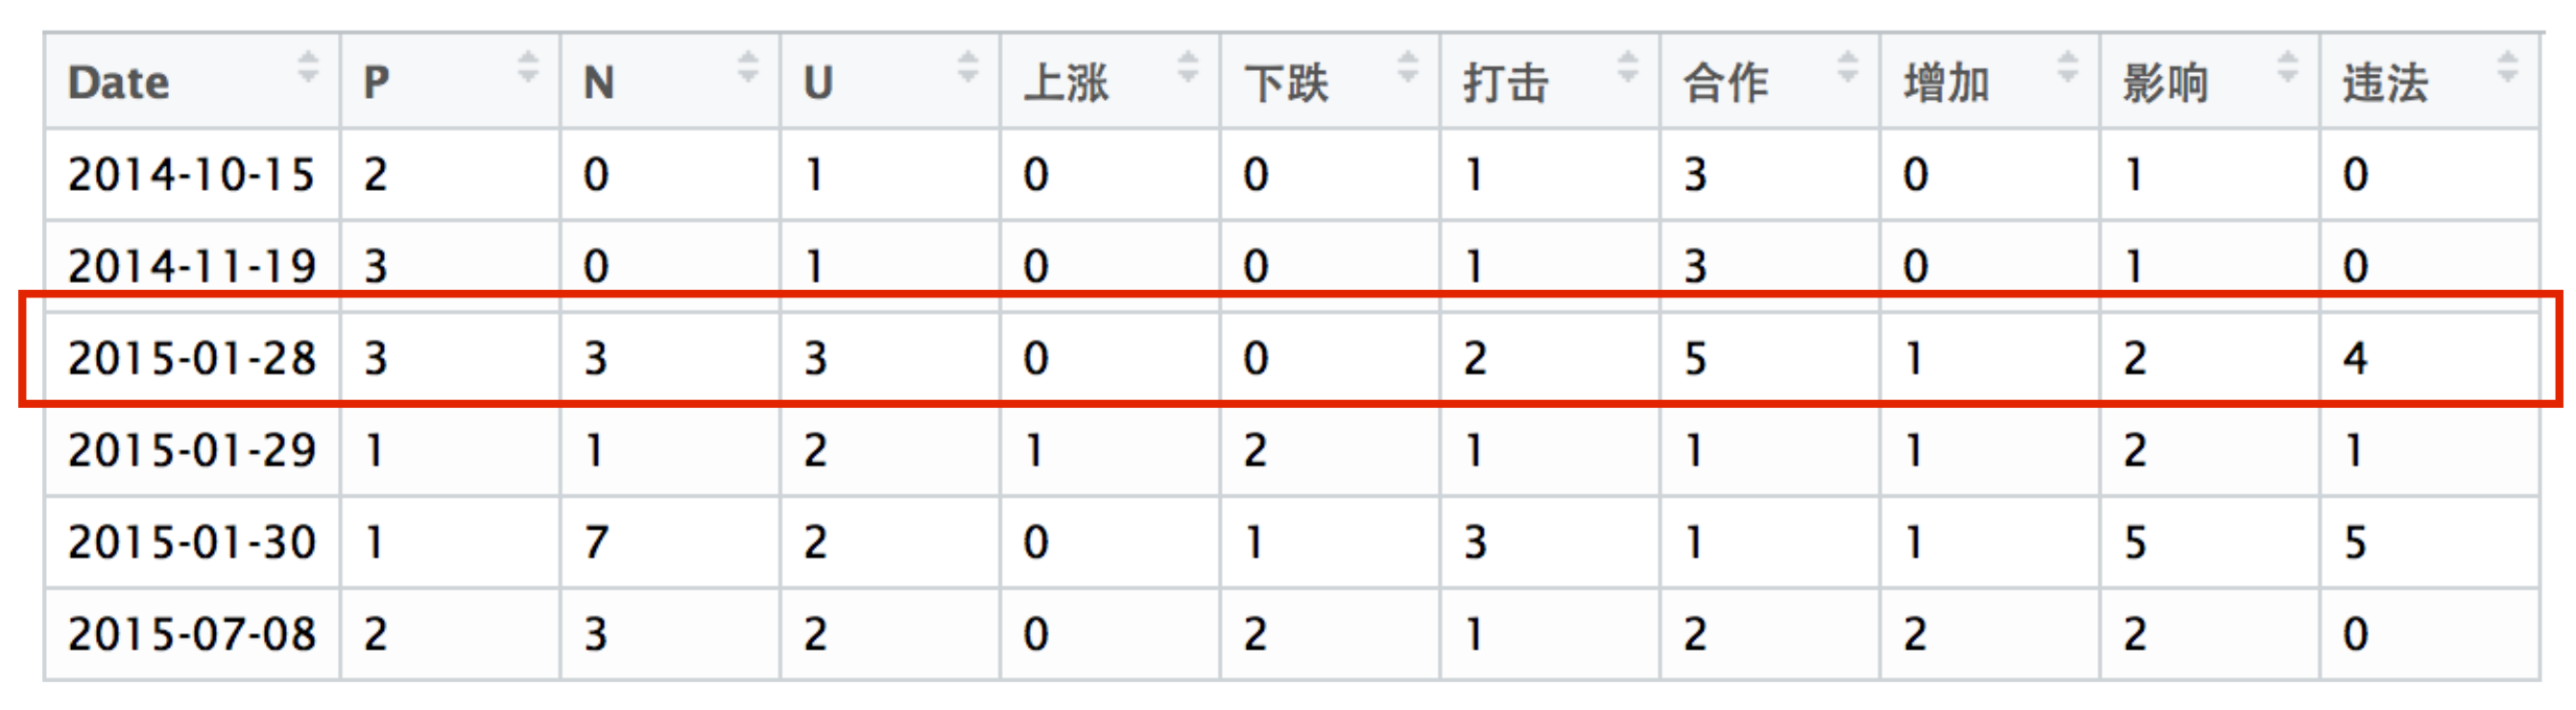
\includegraphics[width=0.55\textwidth]{TextsCovs-New}\\
    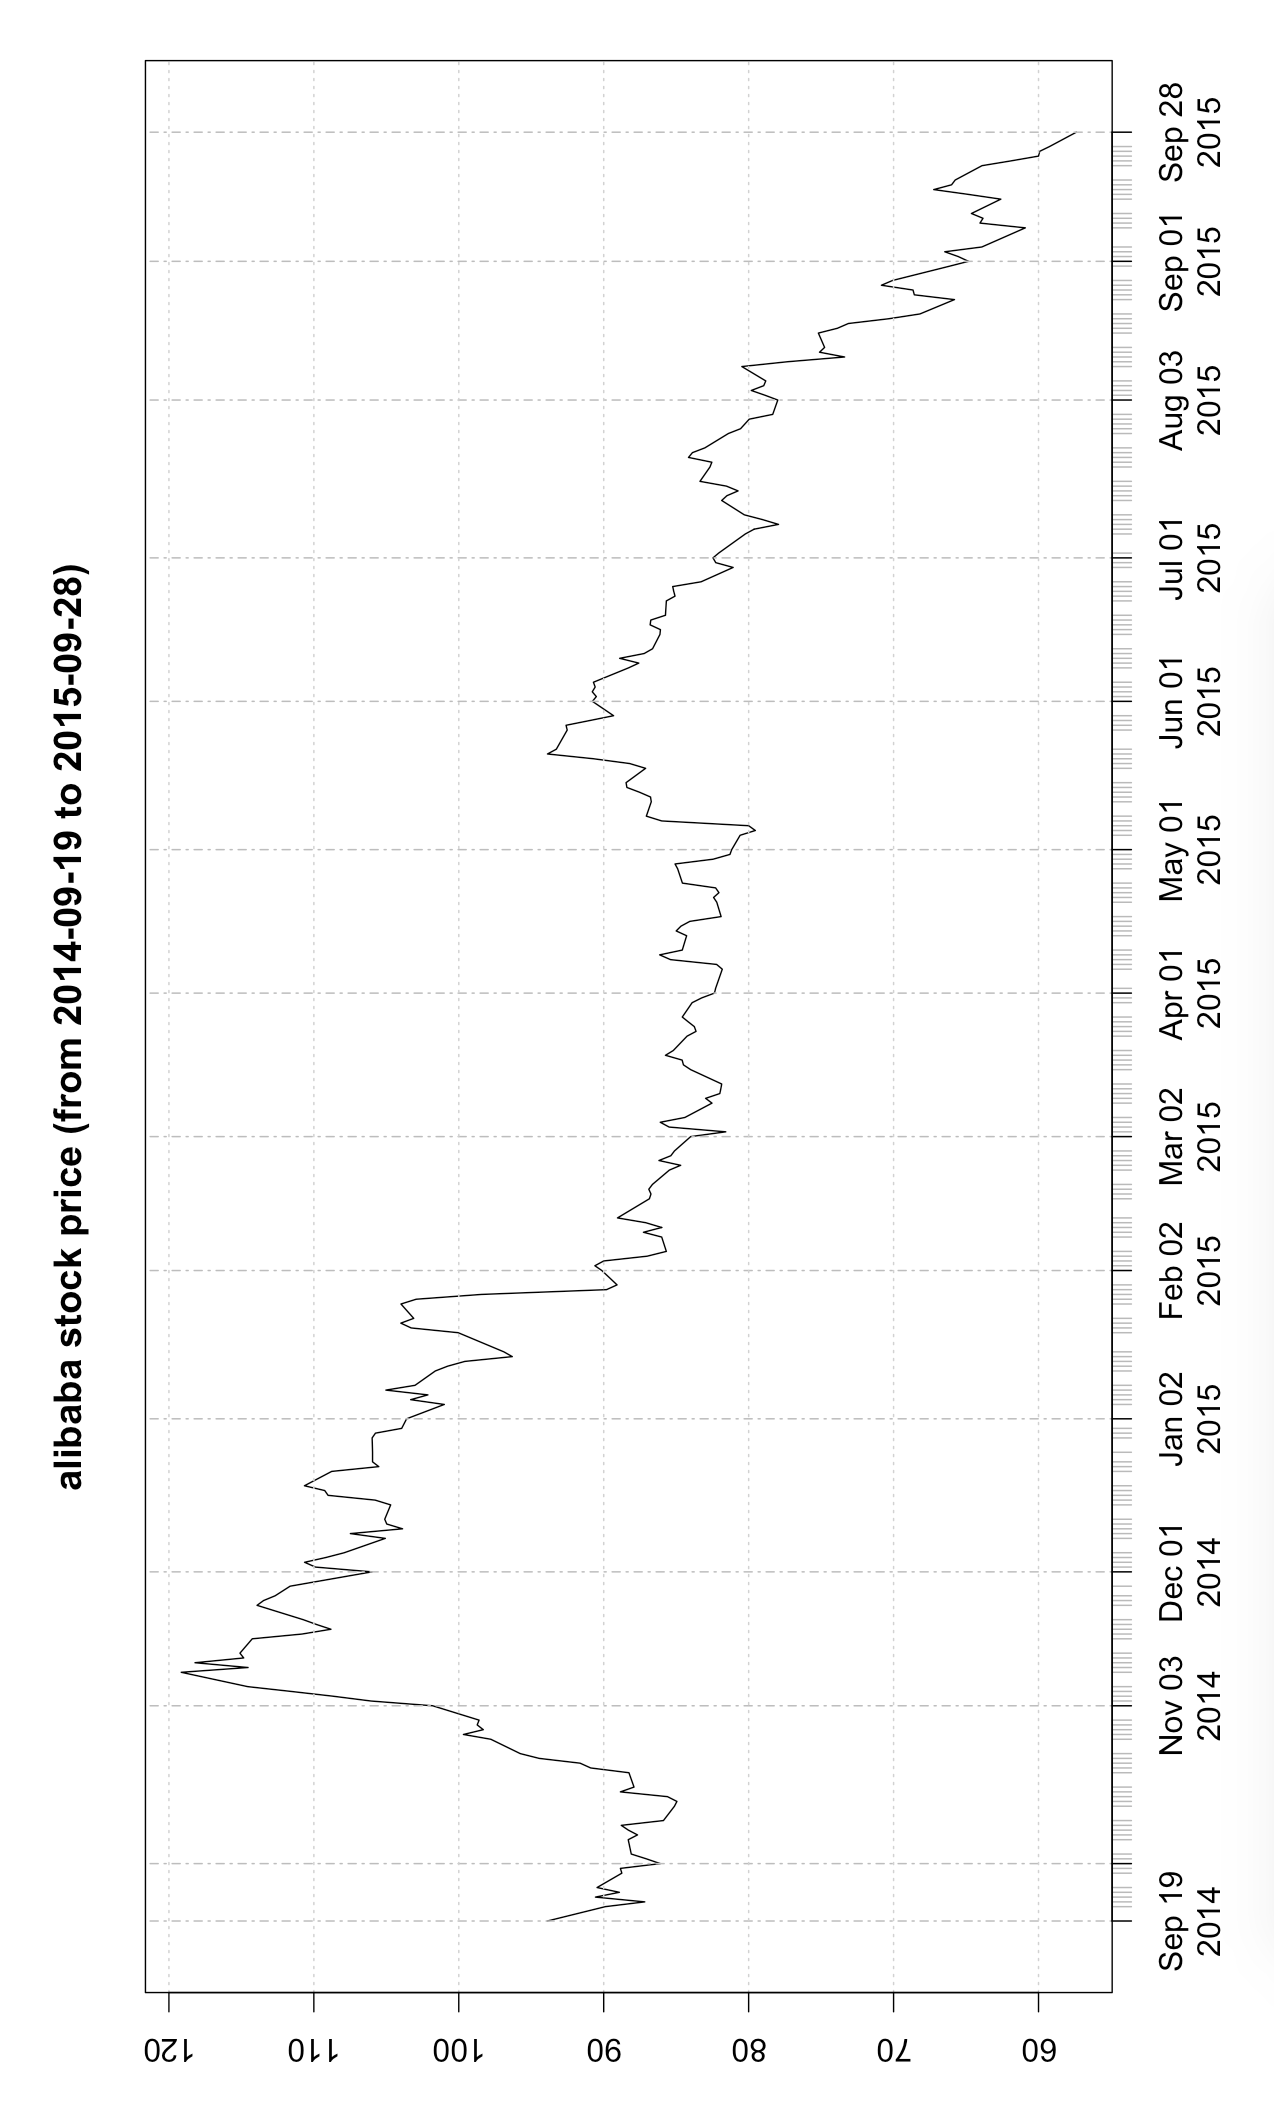
\includegraphics[width=0.27\textwidth]{Alibaba-Stock-Price-R}
    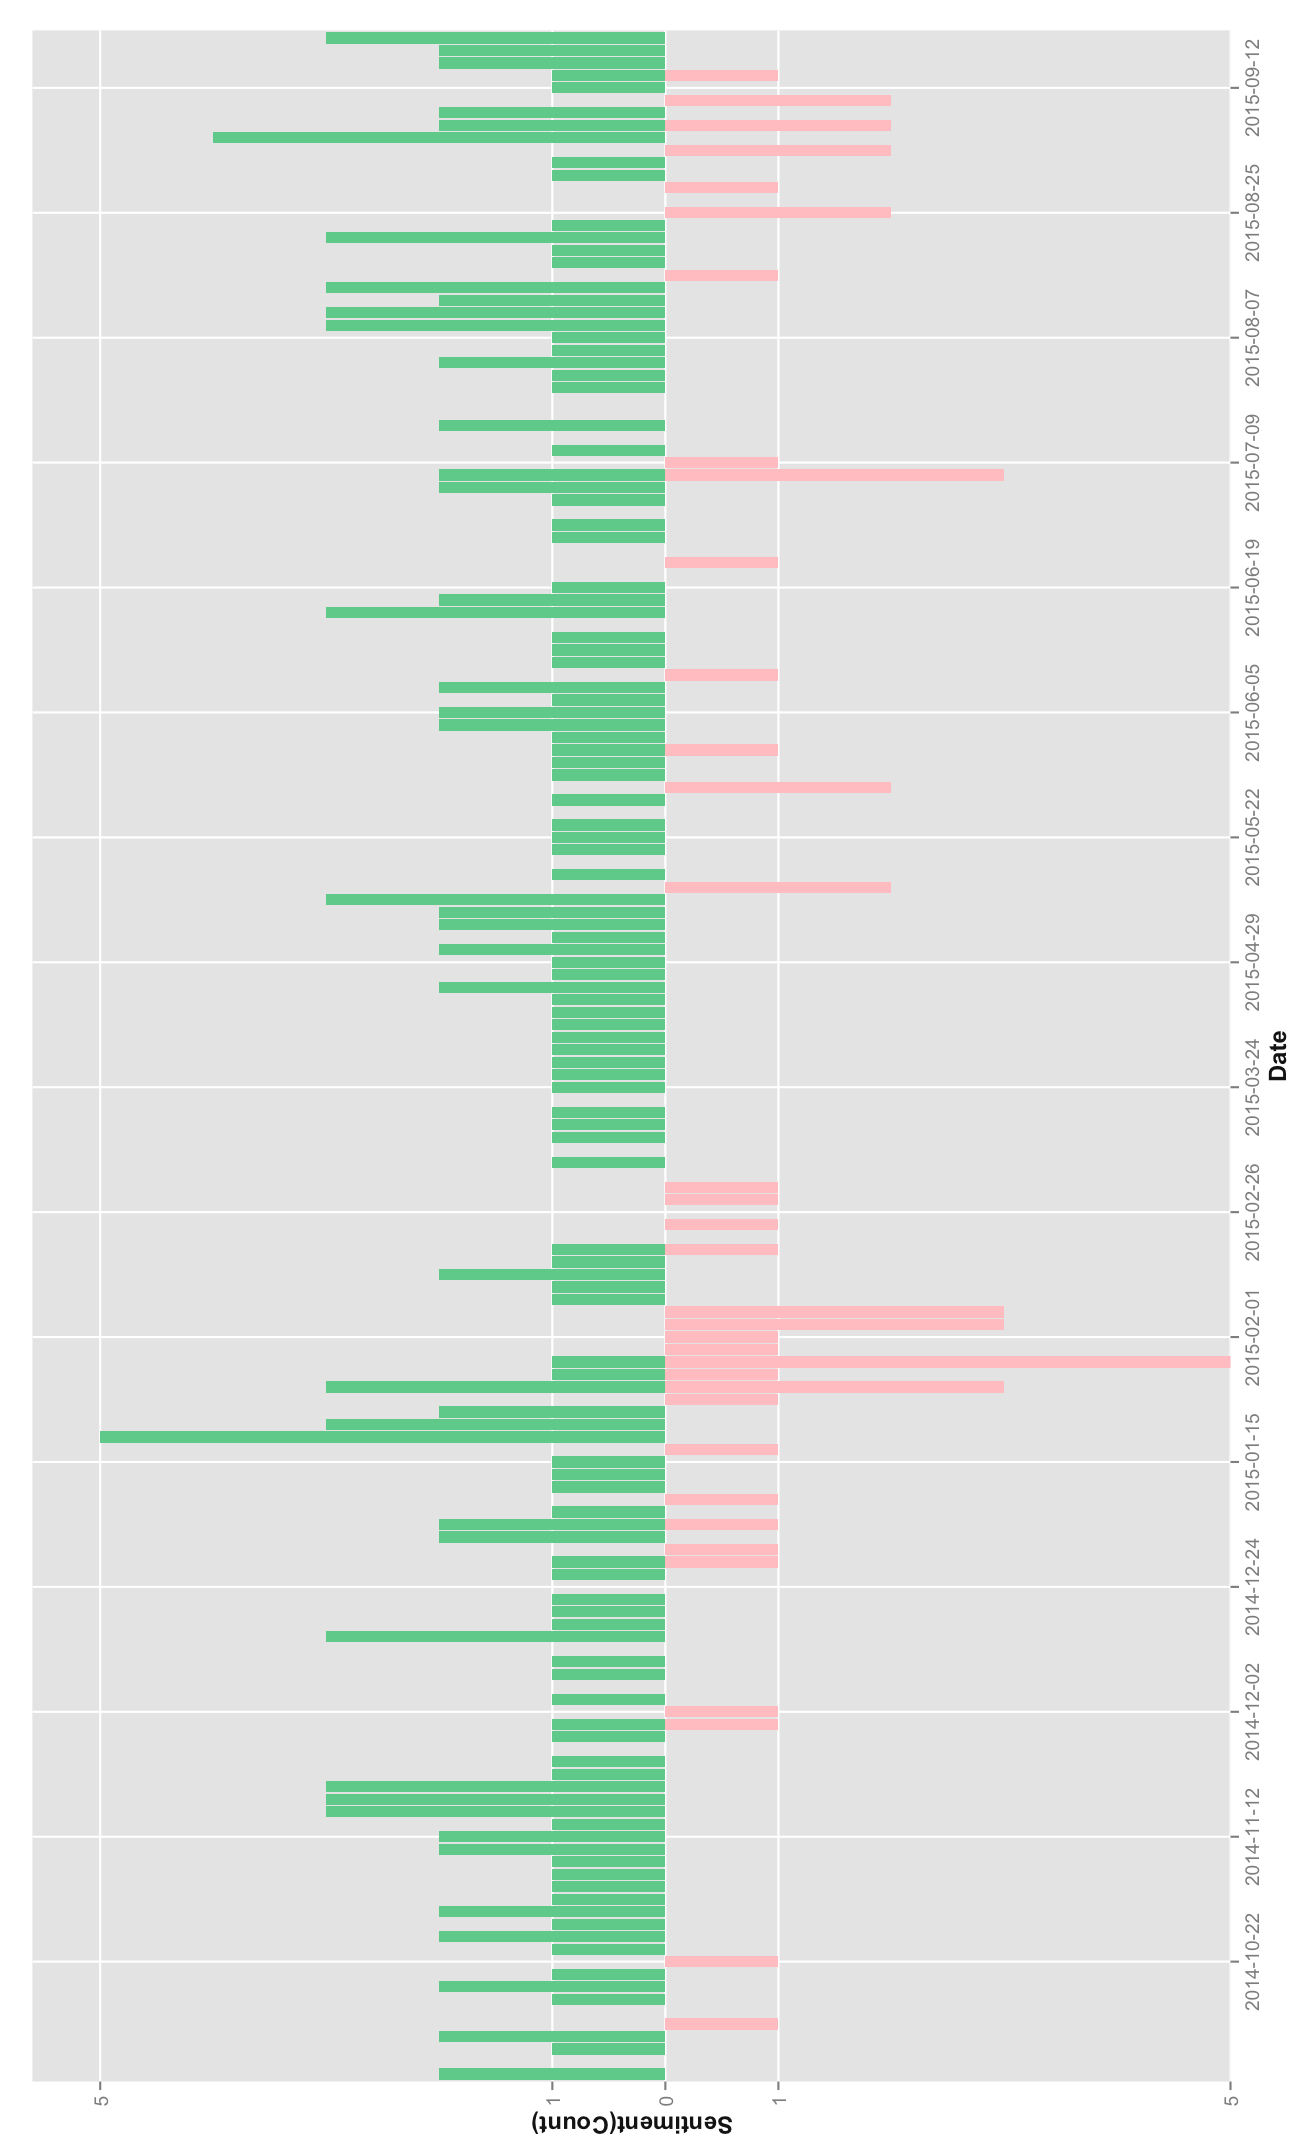
\includegraphics[width=0.27\textwidth]{Sen-Date-R}
  \end{figure}



\end{frame}


\begin{frame}
  \frametitle{Covariates in texts data}
  \begin{figure}
    \centering
    
\includegraphics[width=0.6\textwidth]{Caixin}\\
    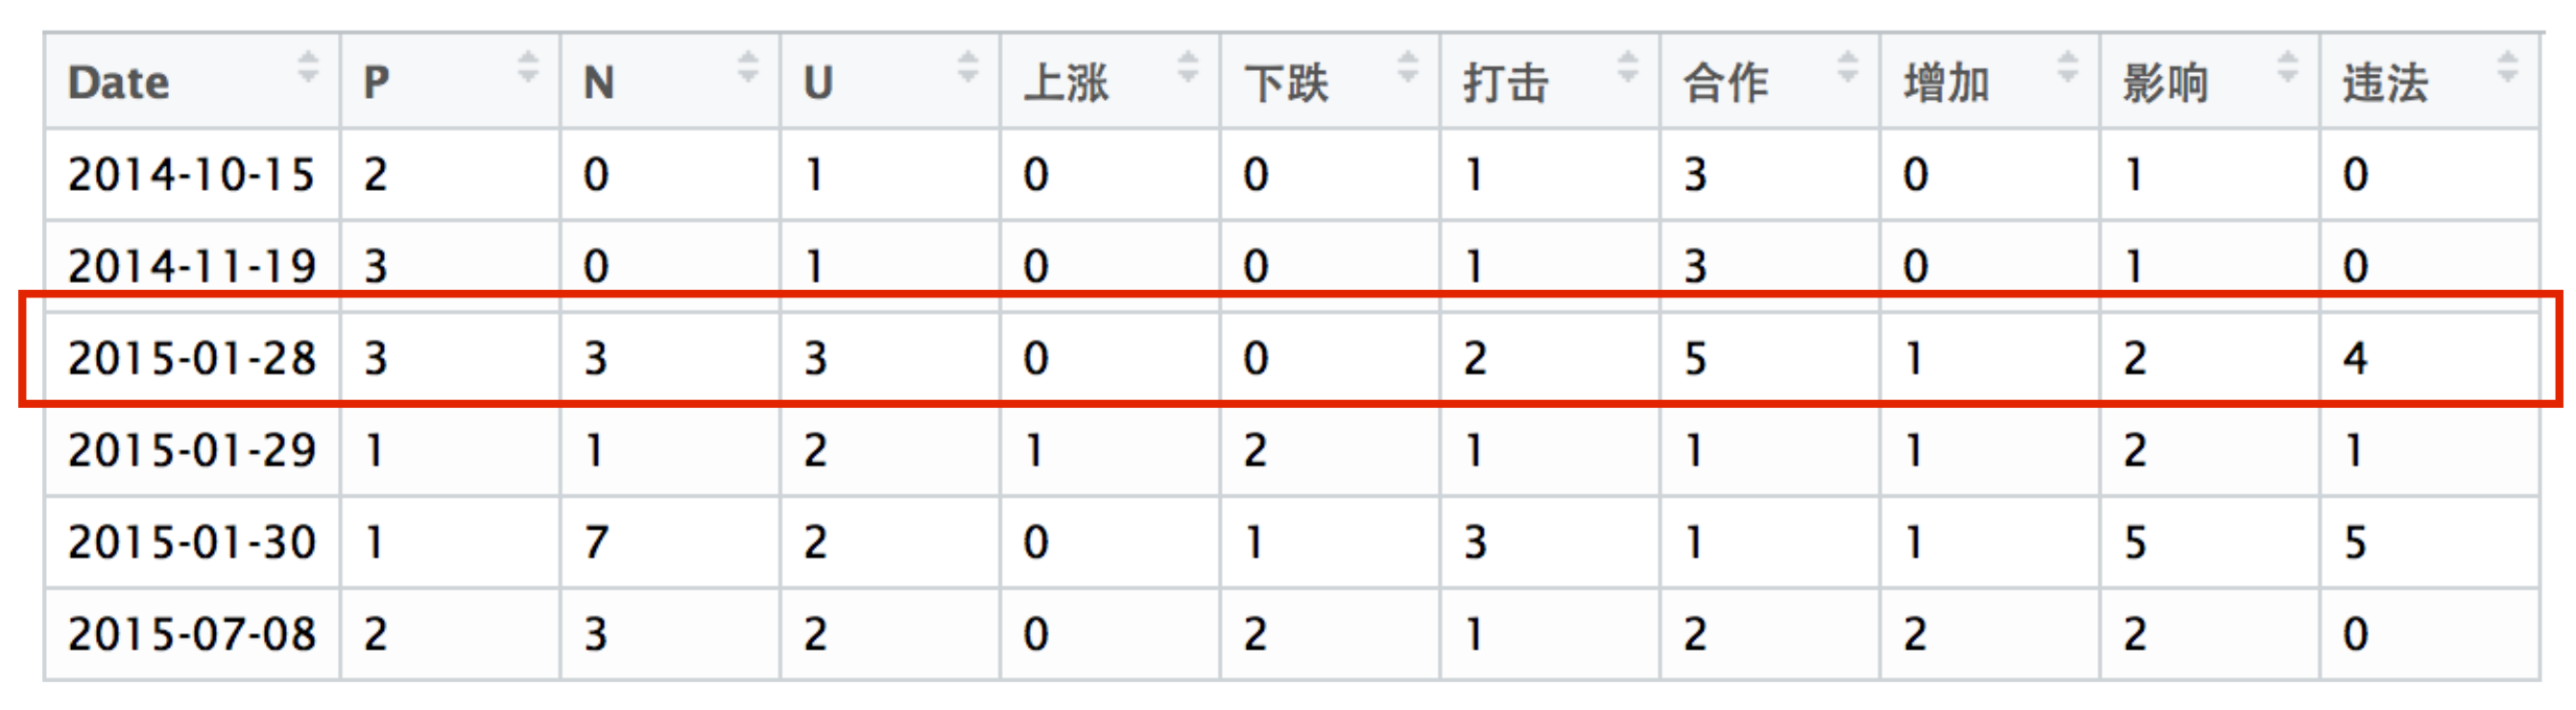
\includegraphics[width=0.6\textwidth]{TextsCovs-New}
  \end{figure}
\end{frame}


\begin{frame}
  \frametitle{The dependence between positive/negative sentiments and stocks}

  \begin{figure}
    \centering
    \includegraphics[width=0.45\textwidth]{BABAlambdaLU}
  \end{figure}

\end{frame}
\begin{frame}
  \frametitle{Working in progress }

  \begin{itemize}
  \item Modeling multivariate covariate-dependent structure via the vine copula.
  \item Looking into more efficient inference techniques, VB?
  \item Including probabilistic topic model to model the texts margins.
  \end{itemize}
\end{frame}


% \begin{frame}[allowframebreaks]
%   \frametitle{References}
%   \bibliography{References,full}
%   \bibliographystyle{asa}
% \end{frame}
\begin{frame}[plain]
  \addtocounter{framenumber}{-1}
  \begin{center}
    {\color{SUblue} \textbf{\Huge Thank you!}}
    \vspace{1cm}

    \url{feng.li@cufe.edu.cn}

    \vspace{1cm}

    \url{http://feng.li/}

  \end{center}
\end{frame}

\end{document}
